\section{Synthetic examples}\label{sec:examples}
The following synthetic examples show how the restrictions affect model choice and the size of approximation errors. All parameters are specified below; the accompanying script generates the figures and table without market data.

\subsection{A distributional distinction with a small curve effect}
Figure~\ref{fig:jumps} uses Example~\ref{ex:binary} with $\pi=1/2$, $\Delta=0.0025$, and maturities out to one year. The level shock is either zero or 25 basis points. The two admissible profiles agree to first order at the origin. Their difference at one year is only about $8.14\times10^{-9}$ basis points. The right panel evaluates this small difference by a Taylor series to avoid subtraction of almost equal floating-point numbers.

The curve restriction therefore distinguishes the two distributions mathematically, but at this rate scale their corrections are almost indistinguishable numerically. Matching a curve to finite precision can leave substantial uncertainty about the announcement distribution.
\begin{figure}[htbp]
\centering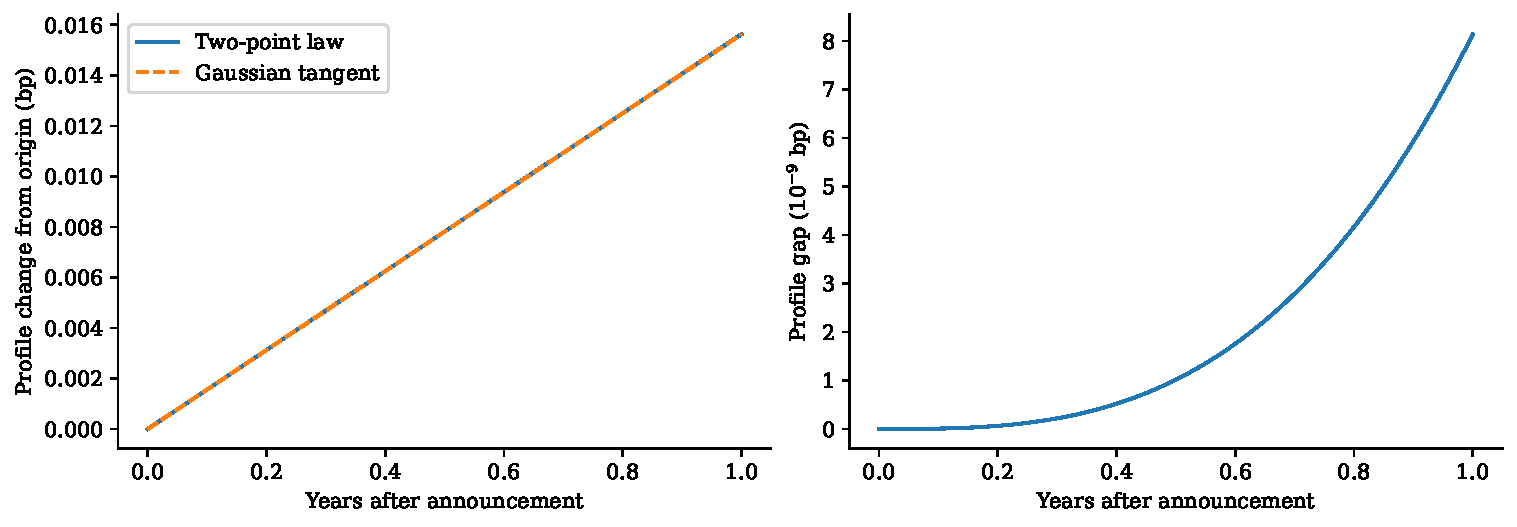
\includegraphics[width=\linewidth]{figures/jump_profiles.pdf}
\caption{Admissible profiles for a symmetric two-point level shock and its Gaussian tangent. The left panel subtracts the common value at zero; the right panel resolves the difference hidden at the scale of the left panel.}\label{fig:jumps}
\end{figure}

\subsection{A small exact recurrent model}
Take $a_i=1-\theta^i$, $0<\theta<1$, and $\lambda(x)=\eta e^{-\kappa x}$. A convenient representation is
\[
u=(1,-1),\quad M=\diag(1,\theta),\quad v=(1,1)^\top,
\qquad c=\eta,\quad A=-\kappa,\quad b=1.
\]
Here $d_*=2$, so \eqref{eq:state} has two $\Xi$ coordinates, three symmetric $\Pi$ coordinates, and two $\Theta$ coordinates. Under constant scale only the two $\Xi$ coordinates are random. Increasing the number of meetings changes $\mathcal D$ and the restart times, but adds no coordinates.

The loadings satisfy $a_{i+2}=(1+\theta)a_{i+1}-\theta a_i$. Their Hankel matrices have rank at most two, and rank exactly two once both independent components are visible. Figure~\ref{fig:hankel} contrasts this example at $\theta=0.7$ with cumulative harmonic loadings. A rapidly falling numerical singular-value spectrum is not a proof of exact finite rank; the distinction between approximation and exact realization is precisely the distinction needed here.
\begin{figure}[htbp]
\centering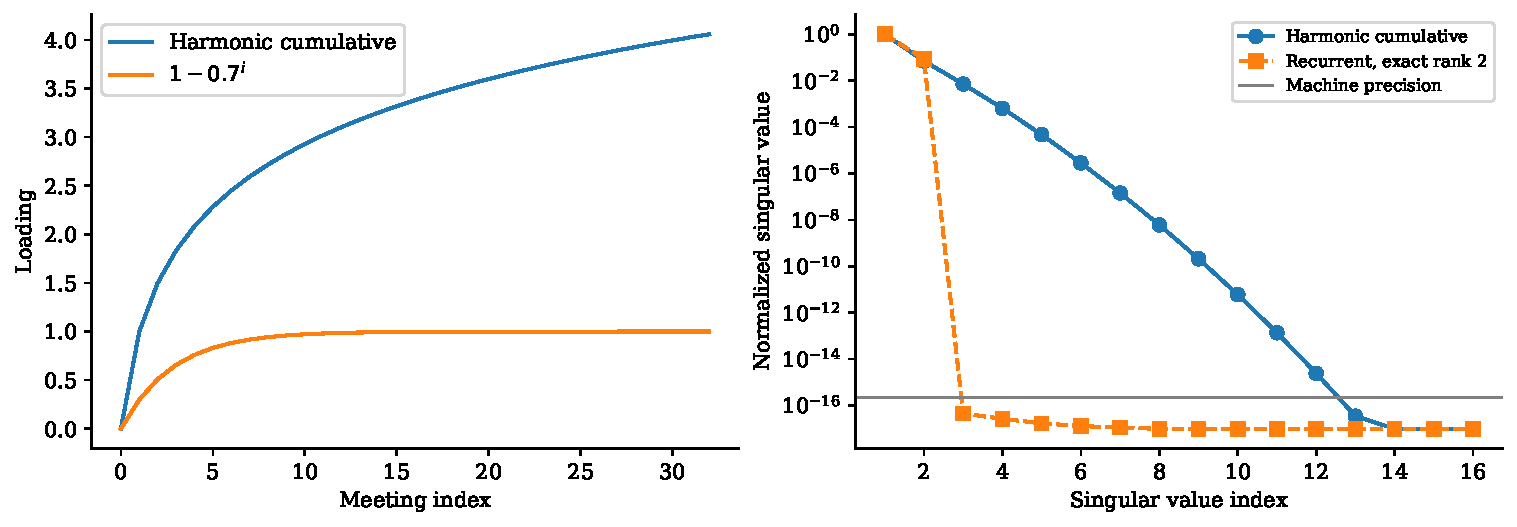
\includegraphics[width=\linewidth]{figures/hankel.pdf}
\caption{Loadings and singular values of their $16\times16$ Hankel sections. The recurrent example has exact rank two. The harmonic sequence is not recurrent, although its finite sections have rapidly decaying singular values. Values close to machine precision should not be interpreted as exact ranks.}\label{fig:hankel}
\end{figure}

\subsection{Compressing harmonic loadings on a calendar}
For integer $i\ge0$,
\begin{equation}
a_i=\sum_{j=1}^i\frac1j=\int_0^1\frac{1-x^i}{1-x}\dd x.
\label{eq:harmonicint}
\end{equation}
Choose $n_q$ Gauss--Legendre nodes $x_j\in(0,1)$ and weights $w_j>0$ on $[0,1]$. The approximation
\begin{equation}
\widetilde a_i=\sum_{j=1}^{n_q}\frac{w_j}{1-x_j}(1-x_j^i)\label{eq:quadraturerecurrence}
\end{equation}
is a sum of a constant and $n_q$ geometric sequences. It therefore has recurrence order at most $n_q+1$, and is bounded as $i\to\infty$ for each fixed $n_q$. The polynomial identity in \eqref{eq:harmonicint} also explains why the first few entries are particularly accurate. The example chooses the number of quadrature nodes and measures the resulting error on the calendar of interest.

Use a four-year horizon with 32 equally spaced meetings strictly inside it, zero initial curve, and $\lambda(x)=0.0025e^{-0.35x}$. Compare forward and bond prices at $t=2$, $T=4$. The maximum loading error is computed over indices $0$ through $32$; Theorem~\ref{thm:approximation} converts it into forward and price bounds. Here we use the sharper pointwise bounds at the chosen observation time and maturity. Table~\ref{tab:approx} compares those bounds with the pointwise Gaussian errors. Forward errors are in basis points of rate; bond errors are $10^4$ times absolute price errors for unit notional.

\begin{table}[htbp]\centering\small
\begin{tabular}{rrrrrr}
\toprule
Order & $\varepsilon$ & Forward RMSE & Bound & Bond RMSE & Bound\\
\midrule
\csname @@input\endcsname examples/results.tex 
\bottomrule
\end{tabular}
\caption{Recurrent approximation on the specified 32-meeting calendar. Orders are upper bounds. Both the bounds and the measured errors are evaluated at $(t,T)=(2,4)$.}\label{tab:approx}
\end{table}

The maturity integrals are evaluated analytically on each meeting interval. Remaining deterministic time integrals use Gauss--Legendre quadrature split at meetings; doubling from 12 to 24 nodes per interval checks numerical convergence. The errors use Gaussian moment formulas, not Monte Carlo estimates. In particular, write the Gaussian log prices as $\ell_P=\log P$ and $\widetilde\ell_P=\log\widetilde P$. Set $\delta_P=\ell_P-\widetilde\ell_P$, $v_P=\Var\delta_P$, and $b_P=\E\delta_P+v_P/2+2\Cov(\delta_P,\widetilde\ell_P)$. Then
\[
\E(P-\widetilde P)^2
 =e^{2\E\widetilde\ell_P+2\Var\widetilde\ell_P}
 \{(e^{b_P}-1)^2+e^{2b_P}(e^{v_P}-1)\}.
\]
Using \texttt{expm1} in this expression avoids cancellation when the approximation is accurate.

\begin{figure}[htbp]
\centering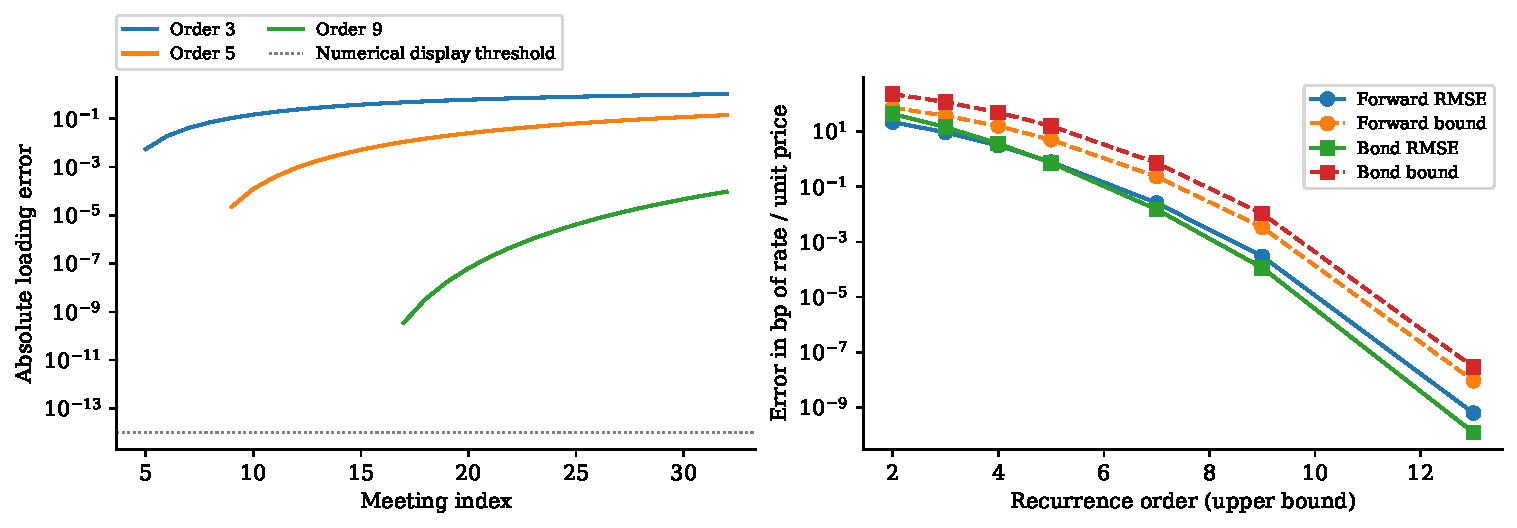
\includegraphics[width=\linewidth]{figures/approximation.pdf}
\caption{Loading approximation and resulting Gaussian forward and bond errors. Dashed curves are the bounds of Theorem~\ref{thm:approximation}; solid curves are computed pointwise errors. Loading errors below $10^{-14}$ are omitted and the numerical display threshold is marked. The comparison uses a fixed finite index range.}\label{fig:approximation}
\end{figure}

\subsection{A forbidden correlation made visible}
Consider a front-end volatility with one step of size $\Delta s$ at $\tau$, and an exponential block volatility $\eta_B e^{-\kappa(T-u)}$, with driver correlation $\rho$. Their aggregate step covariance is $\rho \eta_B\Delta s$, which violates \eqref{eq:steporth} when nonzero. For an observation time $t<\tau$, the difference of the adjacent analytic cross-term extensions, integrated from time zero to $t$, is
\begin{equation}
\mathcal R_\rho(T)=c_\rho e^{-\kappa T}(T-\tau-1/\kappa)+\rho \eta_B\Delta s\,t/\kappa,
\qquad c_\rho=\rho \eta_B\Delta s\frac{e^{\kappa t}-1}{\kappa}.\label{eq:numericcross}
\end{equation}
It is not affine when the covariance is nonzero. Figure~\ref{fig:splice} uses $t=0.5$, $\tau=1$, $\kappa=0.6$, $\eta_B=0.008$, $\Delta s=0.007$, and $\rho=0.6$. Subtracting the affine tangent at the meeting leaves a curved remainder. The remainder displays the shape that a piecewise-linear drift cannot absorb. Thus the figure diagnoses why this proposed correlation is incompatible with the chosen curve family.
\begin{figure}[htbp]
\centering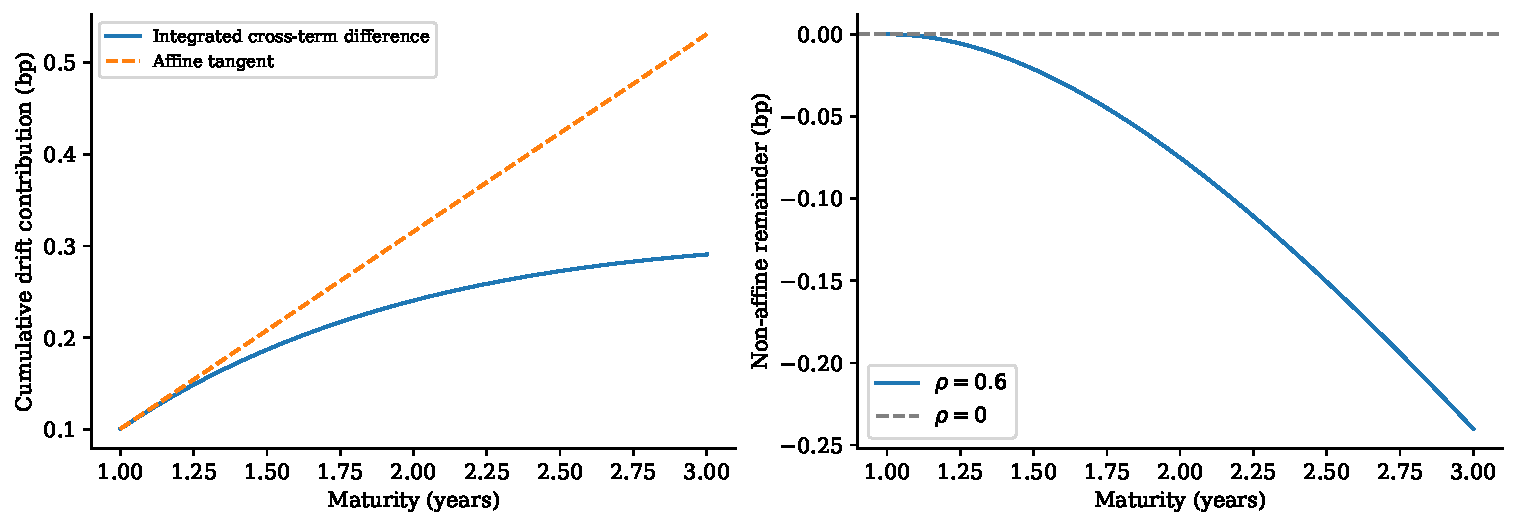
\includegraphics[width=\linewidth]{figures/splice_correlation.pdf}
\caption{A correlation that the stipulated splice cannot accommodate. The residual curvature vanishes when $\rho=0$. A smooth global block and an intervalwise affine front end cannot absorb different non-affine analytic expressions on adjacent intervals.}\label{fig:splice}
\end{figure}

For an eventual fitting procedure, the structural order is clear: choose an admissible block and recurrence class, enforce their covariance restrictions, compute each model's HJM drift, and only then fit loading and scale parameters. The resulting fit would then measure approximation within a class whose dynamics satisfy the structural restrictions.
